%%%%%%%%%%%%%%%%%%%%%%%%%%%%%%%%%%%%%%%%%%%%%%%%%%%%%%%%%%%%%%%%%%% 
%                                                                 %
%                          Uitwerking                             %
%                                                                 %
%%%%%%%%%%%%%%%%%%%%%%%%%%%%%%%%%%%%%%%%%%%%%%%%%%%%%%%%%%%%%%%%%%% 

\chapter{Uitwerking}

\begin{figure}[!h]
    \centering
    \includegraphics[width=\linewidth]{uitwerking/pipeline1.png}
    \caption{Overzicht van het programma}
    \label{fig:pipeline1}
\end{figure}

Het doel van deze masterproef is om op basis van 1 \gls{rgb} camera en een semantische kaart een robot autonoom te laten navigeren in de logistieke gangen van een ziekenhuis.
Om dit te implementeren, stelden we een pipeline op. Een schematische voorstelling van de pipeline is voorgesteld in figuur~\ref{fig:pipeline1} en~\ref{fig:pipeline2}.
Deze pipeline is onderverdeeld in 5 stappen.
Eerst worden er door middel van een object detector (\ref{sec:object_detectie}) visuele kenmerken in de beelden gezocht.
Vervolgens zoeken we het perspectiefpunt in de input frames (\ref{sec:perspectiefpunt_detectie}).
Als derde stap representeren we op basis van de gedetecteerde objecten, en het vluchtpunt de waargenomen kenmerken (\ref{sec:omgevingsmeting}) uit het beeld door middel van hoeken.
Als laatste stap proberen we de locatie van de robot te volgen (\ref{sec:lokalisatie}) door middel van de semantische kaart (\ref{sec:sem_kaart}) en de omgevingsmeting uit de vorige stap.

De implementatie is geprogrammeerd in Python 3.7. De versies van de belangrijkste bibliotheken die gebruikt zijn, zijn weergegeven in tabel~\ref{tab:versies}.

\begin{table}
    \centering
    \caption{Belangrijkste Python bibliotheken en versienummers}
    \label{tab:versies}
    \begin{tabular}{l|l|l|l}
        \textbf{Bibliotheek} & OpenCV & Osmnx & Tensorflow \\
        \hline
        \textbf{Versie} & 3.4.5 & 0.9 & 1.13.1 \\
    \end{tabular}
\end{table}


\section{Object detectie}\label{sec:object_detectie}

Zoals besproken zal worden in hoofdstuk~\ref{sec:sem_kaart}, bevat de semantische kaart van het ziekenhuis een beschrijving van objecten/features die aanwezig zijn in de gangen.

De object detector die we gekozen hebben is YOLOv2\cite{yolov22016}.
Dit is een zeer veel gebruikt object detectie/classificatie convolutioneel neuraal netwerk dat toelaat om objecten van een geleerde klasse te herkennen en lokaliseren in nieuwe beelden.
De belangrijkste reden dat we deze detector gekozen hebben, is omdat op een grafische kaart deze real-time kan werken.

\subsection{Datasets}
De gebruikte dataset zijn 2 video's opgenomen vanop een robot met de de waylens horizon\footnote{https://waylens.com/horizon/techSpecs/} \gls{rgb} dashboard camera.
De camera heeft een resolutie van 1920x1080 pixels en filmt met een framerate van 30Hz.
Wij hebben voor training en test de video verdeeld in afzonderlijke frames met een resolutie van 1280x720 pixels waarbij we slechts
aan 15Hz gesampled hebben.

In dit beeldmateriaal zijn volgende features zichtbaar:
\begin{itemize}
    \item Lampen;
    \item Rookdetectors;
    \item Deurklinken;
    \item Nooduitgang bordjes.
\end{itemize}

Zoals eerder besproken bestaat de dataset uit 2 delen, een trainingsset en een validatieset.
De twee sets zijn twee opeenvolgende video's van dezelfde gang uit een ziekenhuis.
De trainingsvideo is hierbij het 2de deel van de gang, en de validatievideo het startpunt.

Het aantal beelden en objecten dat we ter beschikking hebben, is weergegeven in tabel~\ref{tab:annotaties}.

\subsection{Annotatie beeldmateriaal}
Om een object-detector te maken gebaseerd op een \gls{cnn} moet al het beeldmateriaal geannoteerd worden door bounding-boxes te teken rondom de kenmerkende objecten.
Elk van deze bounding-boxes moet ook voorzien worden van een bijhorend label.
Er is gekozen om de dataset op te splitsen in 2 delen, een training en een validatie set.
De 2 datasets omvatten verschillende delen van de gangen in het gebouw.
Het splitsen is nodig om door middel van de validatie set te valideren hoe goed de detector presteert op niet eerder geziene beelden.
In tabel~\ref{tab:annotaties} is een opsomming gemaakt van alle annotaties in de training en validatie set.

\begin{table}[h]
    \caption{Annotaties in training en validatie set}\label{tab:annotaties}
    \begin{tabular}{l | l | l | l | l | l | l}
        & Aantal frames & Rookmelder & Deurklink & Pictogram & TL-lamp & Totaal \\ \hline
        Trainingsset & 899 & 1016 & 147 & 340 & 5260 & 6763 \\
        Validatieset & 711 & 1130 & 180 & 408 & 992 & 2710 \\
    \end{tabular}
\end{table}

Voor het aanduiden van de annotaties maakten we gebruik van de OpenCV \gls{cvat}\footnote{https://github.com/opencv/cvat}.
De output van de \gls{cvat} tool is een XML-bestand met voor elke afbeelding de co\"{o}rdinaten van de objecten. Een voorbeeld output voor 1 enkele afbeelding is te zien in listing~\ref{lst:cvat_xml}.

\lstset{language=XML, caption={Voorbeeld CVAT output}, label={lst:cvat_xml}}
   \begin{lstlisting}[basicstyle=\small]
<image id="24" name="hospital_corridors_025.png" width="1280" height="720">
   <box label="door_handle" xtl="863" ytl="237" xbr="881" ybr="248"/>
   <box label="light" xtl="584" ytl="254" xbr="608" ybr="265"/>
   <box label="light" xtl="435" ytl="321" xbr="448" ybr="329"/>
   <box label="exit_sign" xtl="590" ytl="298" xbr="604" ybr="307"/>
</image>
   \end{lstlisting}

De trainingsdata die aan het \gls{yolo} netwerk geleverd moet worden is in een ander formaat dan het verkregen XML bestand, daarom hebben we een conversiescript geschreven om dit om te zetten naar het \gls{yolo} formaat.
Het formaat dat \gls{yolo} verwacht is per input afbeelding een .txt bestand met daarin per lijn een bounding box. Het \gls{yolo} formaat is beschreven in~\ref{eq:yolo} waarbij $<x>$ en $<y>$ het centerpunt van een bounding box zijn.
Alle waarden zijn genormaliseerd, dit wil zeggen dat om het absolute $(x, y)$ co\"{o}rdinaat te bekomen, de waardes vermenigvuldigd moeten worden met de breedte en de hoogte zoals ge\"{i}llustreerd in~\ref{eq:yolo_abs}.

\begin{equation} \label{eq:yolo}
  <x> <y> <width> <height>
\end{equation}

\begin{equation} \label{eq:yolo_abs}
    \begin{split}
        x_{abs} &= <x> \cdot  image\_width \\
        y_{abs} &= <y> \cdot image\_height
    \end{split}
\end{equation}


\subsection{Training YOLOv2}

Voor training en later ook detectie met YOLOv2 is er gebruikt gemaakt van een aangepaste versie van de darknet\footnote{https://github.com/AlexeyAB/darknet} implementatie in C.
We zijn vertrokken van het yolo-voc.2.0.cfg configuratiebestand waar we het aantal te detecteren klassen hebben aangepast naar 4 (light, smoke\_detector, exit\_sign en door\_handle), en het aantal filters naar 25.
Dit nieuw configuratiebestand specificeert de netwerklayout, deze layout is een YOLOv2 netwerk waarbij nu de laatste lagen aangepast zijn om slechts 4 objecten te classificeren.
De belangrijkste parameters zijn weergegeven in tabel~\ref{tab:hyperparameters}.

Het trainen gebeurt nu op basis van de trainingsset zoals weergegeven in tabel~\ref{tab:annotaties}. De performantie van het netwerk zal besproken worden in hoofdstuk~\ref{ch:resultaten}.

\begin{table}[h]
    \centering
    \caption{YOLOv2 training hyperparameters} \label{tab:hyperparameters}
    \begin{tabular}{l | l | l | l | l | l | l}
        \textbf{Naam} & Batch size & Batch subdivisions & Learning rate & Maximum batches & Classes & Filters \\
        \hline
        \textbf{Waarde} & 64 & 8 & 0.0001 & 45000 & 4 & 25
    \end{tabular}
\end{table}


\section{Perspectiefpunt detectie}\label{sec:perspectiefpunt_detectie}

In hoofdstuk~\ref{sec:omgevingsmeting} zullen we bespreken hoe we de locatie van de robot gaan volgen, om dit te realiseren wordt er gebruik gemaakt van het perspectiefpunt.
Het detecteren van het vluchtpunt of perspectiefpunt kan gebeuren op verschillende manieren, voor dit onderzoek hebben we drie verschillende technieken uitgevonden en ge\"{i}mplementeerd, en deze zullen verder besproken worden.

De performantie en nauwkeurigheid van de 3 methoden zal besproken worden in hoofdstuk~\ref{ch:resultaten}.

\subsection{Hoogste vloerpixel segmentatie}\label{sec:seg_highest}

De eerste techniek maakt gebruik van het DeepLab-ResNet~\cite{resnet101} segmentatienetwerk, gelijkaardig aan de beschrijving in hoofdstuk~\ref{sec:image_segmentation}.
Het netwerk is ge\"{i}mplementeerd in TensorFlow en voorgetraind op indoor scenes zodat het klaar is voor gebruik in python.\footnote{https://github.com/hellochick/Indoor-segmentation}

Het netwerk kan gebruikt worden om in een afbeelding elke pixel onder te verdelen in een aantal klassen zoals: muur, vloer, boom, meubel en trap.
Voor het detecteren van het perspectiefpunt hebben we gekozen om enkel de vloerpixels te gebruiken.
Het resultaat van de segmentatie is te zien in figuur~\ref{fig:floor_seg} waarbij groen vloerpixels zijn, roze muurpixels, grijs plafondpixels en blauw meubelpixels.

In eerste instantie nemen we van de gesegmenteerde data de hoogste vloerpixel, en deze gebruiken we als perspectiefpunt.
Dit illustreren we in figuur~\ref{fig:floor_seg}

Deze methode is mooi in theorie omdat het hoogste punt van de vloer het perspectiefpunt zou moeten zijn.
Het probleem is echter dat als de vloersegmentatie niet perfect is, de hoogste pixel op een andere plaats kan liggen.
Als bijvoorbeeld het segmentatie netwerk een deel van de muur hetzelfde classificeert als de vloer, zal dit deel vaak hoger liggen dan het
effectieve perspectiefpunt, en zorgen voor een totaal verkeerde detectie.

\begin{figure}
    \centering
    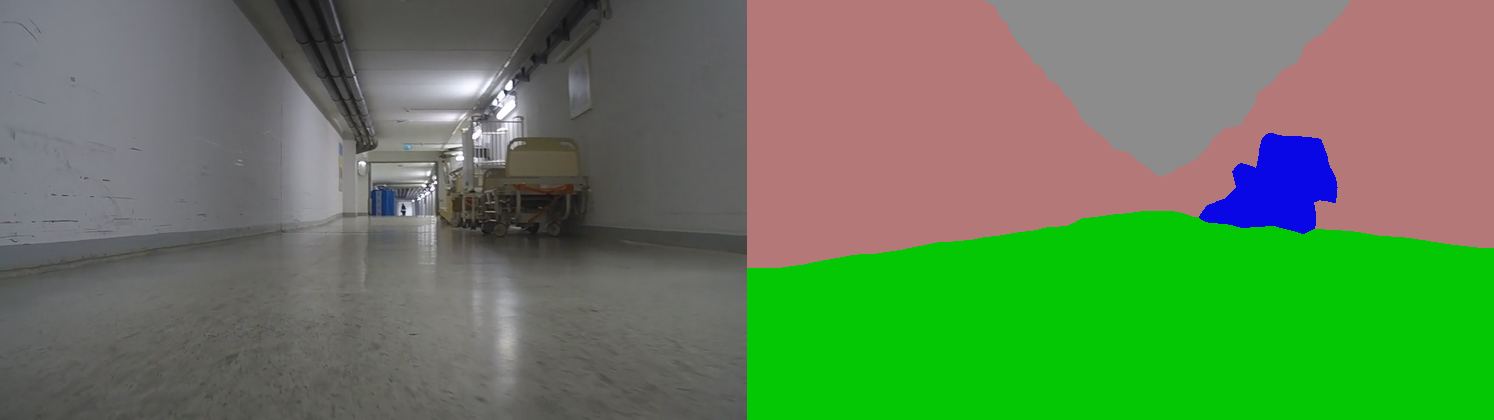
\includegraphics[width=\linewidth]{uitwerking/segmentatie.png}
    \caption{ResNet segmentatie van 1 input frame.}
    \label{fig:floor_seg}
\end{figure}
\begin{figure}
    \centering
    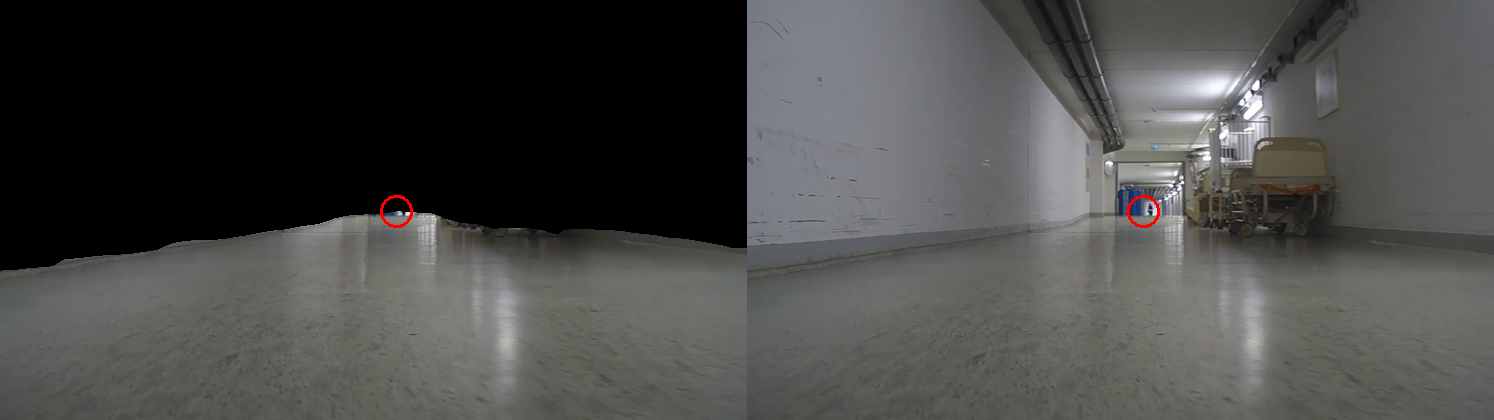
\includegraphics[width=\linewidth]{uitwerking/seg_highest.png}
    \caption{Hoogste vloerpixel als perspectiefpunt}
    \label{fig:highest_pixel}
\end{figure}


\subsection{Vloerlijn kruising}\label{sec:hough_floor}
Voor deze techniek maken we gebruik van dezelfde segmentatiedata als in hoofdstuk~\ref{sec:seg_highest}, maar wordt er een masker gemaakt met enkel de vloerpixels.
Op dit masker wordt door middel van een Canny-edgedetector de rand van de vloer gedetecteerd, dit proces is gevisualiseerd in figuur~\ref{fig:hough_floor}.
Vervolgens kunnen er door middel van de Hough-transformatie een aantal rechten gevonden worden die raken aan zoveel mogelijk punten met de rand van de vloer.
Zoals te zien in figuur~\ref{fig:hough_floor} worden er meerdere rechten gevonden, en deze moeten gefilterd worden omdat ze ongeveer dezelfde lijn voorstellen.
Dit gebeurt door de richtingsco\"{e}ffici\"{e}nt van alle lijnen met elkaar te vergelijken, en indien het verschil te klein is, wordt de lijn met de laagste
richtingsco\"{e}ffici\"{e}nt verwijderd.
Het optimale resultaat is dat er 1 lijn overblijft aan elke kant van de vloer, zodat deze de vluchtlijnen voorstellen.
Indien dit het geval is, is de kruising van de 2 rechten het perspectiefpunt.

Deze techniek werkt goed als de rand van de vloer mooi de perspectieflijnen volgt.
Indien er teveel objecten zoals karren of paletten aanwezig zijn op de vloer, kan dit zorgen voor een grillige vloersegmentatie.
Deze grillige vormen kunnen ervoor zorgen dat de lijnen niet samenvallen met de perspectieflijnen waardoor de kruispunten niet het perspectiefpunt zullen aanduiden.

\begin{figure}
    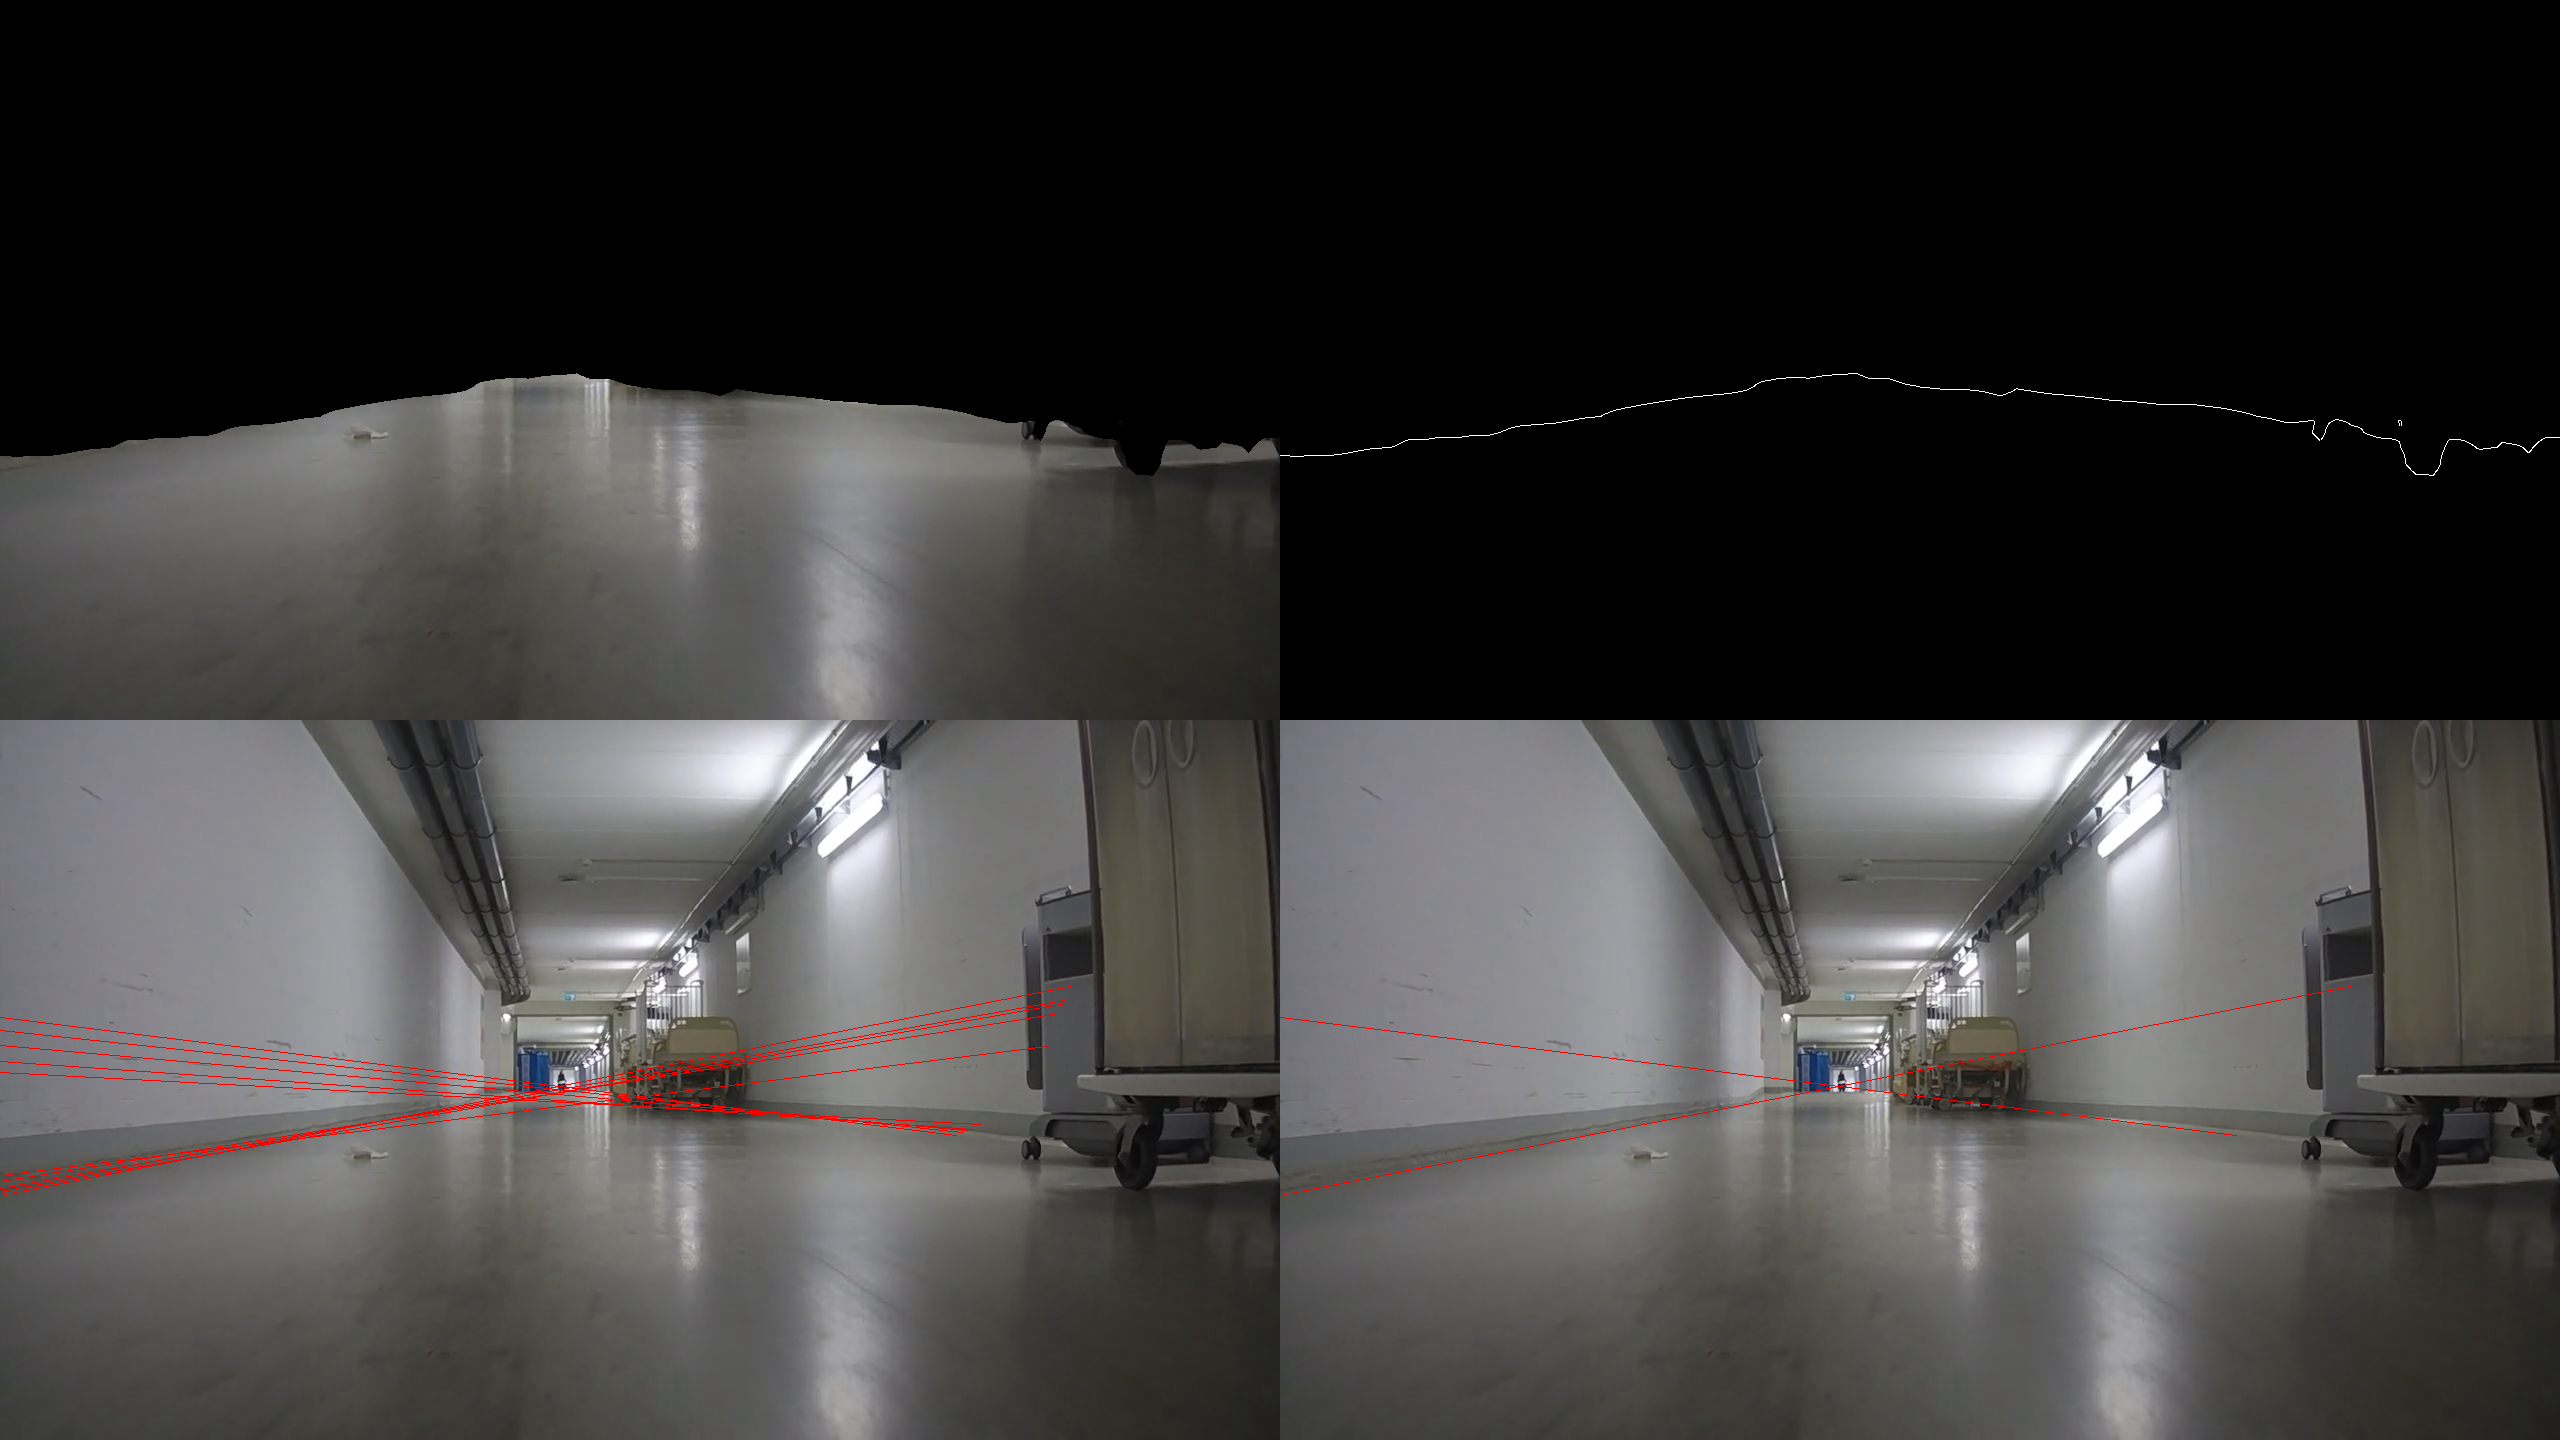
\includegraphics[width=\linewidth]{uitwerking/hough_floor.png}
    \caption{\textbf{Linksboven}: vloersegmentatie, \textbf{Rechtsboven}: Canny-edgedetectie, \textbf{Linksonder}: alle Hough lijnen, \textbf{Rechtsonder}: filtering van lijnen + resultaat}
    \label{fig:hough_floor}
\end{figure}


\subsection{Perspectieflijn kruising}\label{sec:perspectieflijnkruising}
Deze techniek gelijkt sterk op de beschreven methode uit~\ref{sec:hough_floor} met als verschil dat hier geen gebruik gemaakt wordt van vloersegmentatie.
De gehele afbeelding wordt omgezet naar grijswaarden voordat het door een Canny-edgedetector gehaald wordt met een variabele treshold gebaseerd op de mediaan van de grijswaarden.
De edge detectie wordt wederom gebruikt om door middel van de Hough-transformatie een aantal aanliggende rechten te zoeken die zoveel mogelijk punten snijdt.
We zijn op zoek naar perspectieflijnen, dus alle horizontale en verticale lijnen worden onmiddellijk verwijderd net als rechten waarvan de richtingsco\"{e}ffici\"{e}nt
niet genoeg van elkaar afwijkt. Dit is weergegeven in figuur~\ref{fig:hough_all}.

Indien er slechts een paar lijnen overblijven na filtering, kan gesteld worden dat het perspectiefpunt te vinden is op de kruising van de rechten.
In het geval dat er nog meerdere kruispunten zouden overschieten, kan er een gemiddelde positie berekend worden van deze punten.

\begin{figure}
    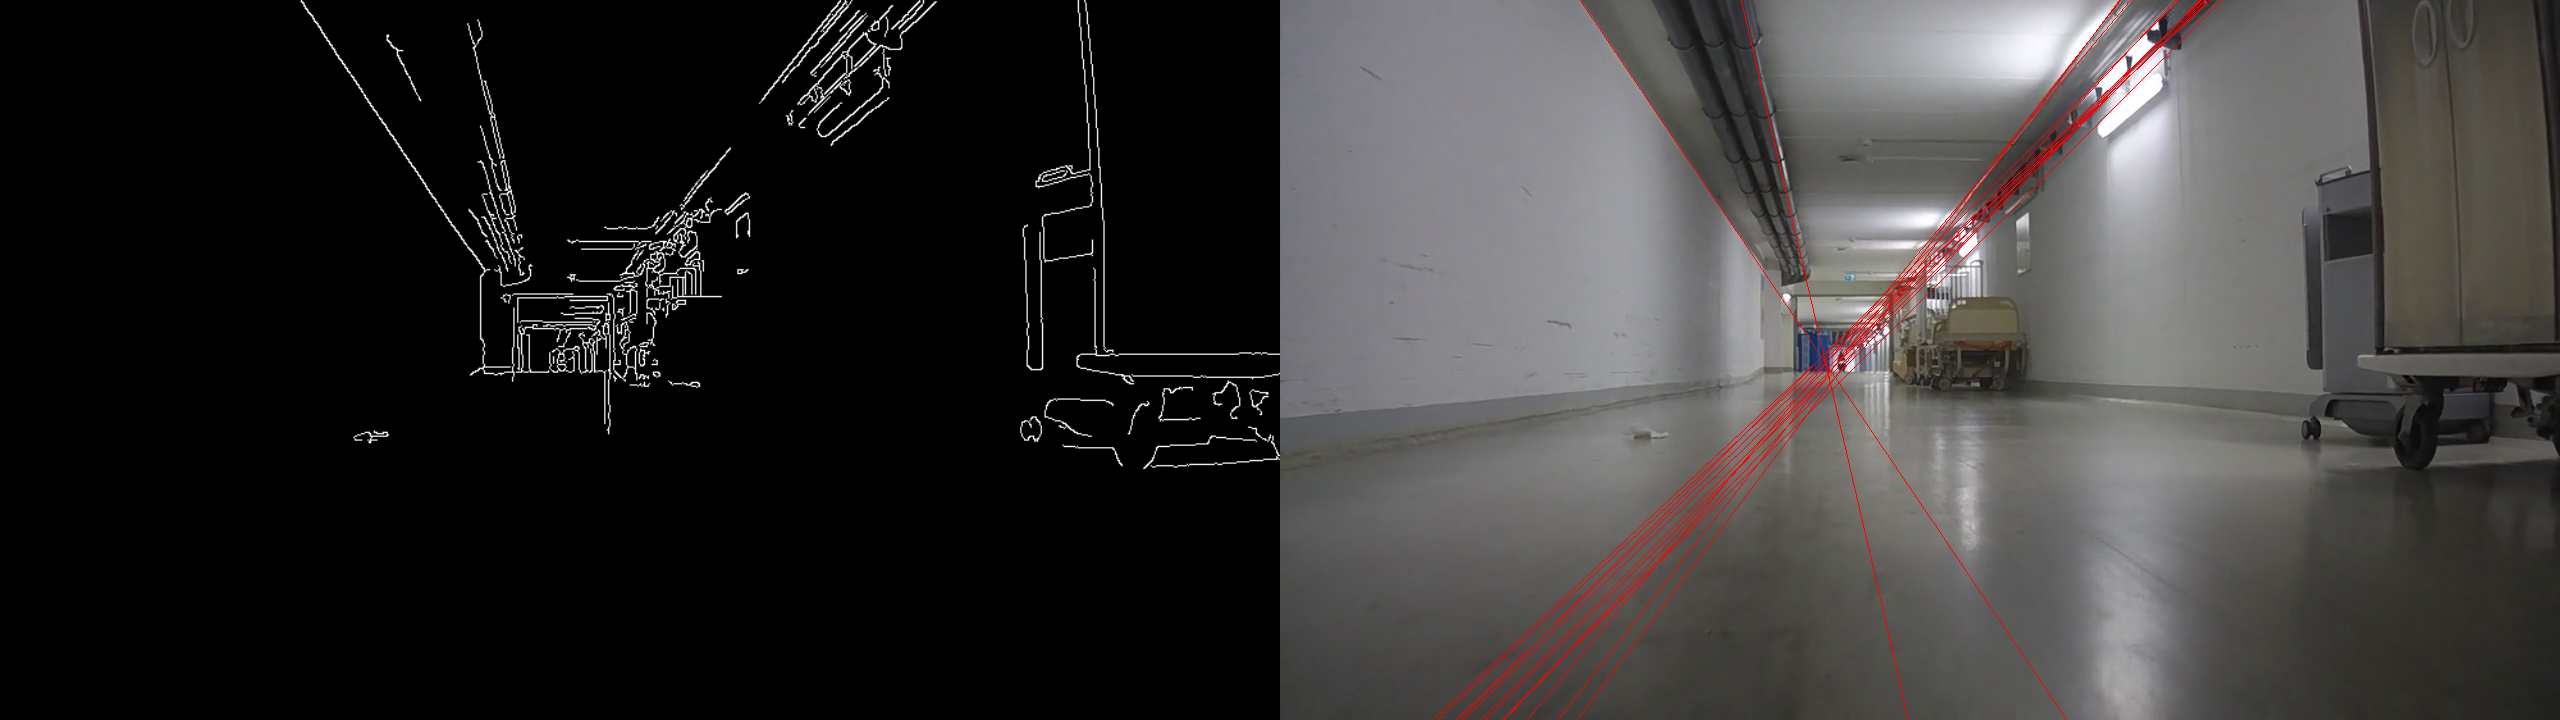
\includegraphics[width=\linewidth]{uitwerking/hough_all.png}
    \caption{\textbf{Links}: Canny-edgedetectie op hele afbeelding. \textbf{Rechts}: Hough lijnen uit edge detection.}
    \label{fig:hough_all}
\end{figure}


\section{Omgevingsmeting} \label{sec:omgevingsmeting}

\begin{figure}[!h]
    \centering
    \begin{tikzpicture}[x=1cm,y=1cm,z=0.6cm,>=stealth]
        \coordinate (Camera) at (-3, 1);
        \coordinate (Obj1) at (0, 3);
        \coordinate (Obj2) at (0, 6);
        \coordinate (Obj3) at (-6, 9);

        % Side lines
        \draw (-6,0) -- (-6,12);
        \draw (0,0) -- (0,12);

        % Objects
        \node[fill,circle, inner sep=2pt, label={right:Obj}] at (Obj1) {};
        \node[fill,circle, inner sep=2pt, label={right:Obj}] at (Obj2) {};
        \node[fill,circle, inner sep=2pt, label={right:Obj}] at (Obj3) {};

        % Camera
        \node[fill,circle,inner sep=2pt, label={left:Camera}] at (Camera) {};

        % Field of view
        \draw[dashed] (-3, 1) -- (0,4);
        \draw[dashed] (-3, 1) -- (-6,4);
        \draw[dashed] (-3, 1) -- (-3,12);

        % Focal plane
        \draw[blue, name path=fplane] (-1, 3) -- (-5, 3);

        % Obj to camera
        \draw[dashed, red, name path=o2--c] (Obj2) -- (Camera);
        \draw[dashed, red, name path=o3--c] (Obj3) -- (Camera);

        \pic [draw, <->, "$\alpha_2$", angle eccentricity=1.1, angle radius=3cm] {angle = Obj2--Camera--Camera};
        \pic [draw, <->, "$\alpha_3$", angle eccentricity=1.1, angle radius=3.5cm] {angle = Camera--Camera--Obj3};

        % Projection points
        \path[name intersections={of=o2--c and fplane,by=p2}];
        \node[fill,circle,inner sep=2pt, red] at (p2) {};
        \path[name intersections={of=o3--c and fplane,by=p3}];
        \node[fill,circle,inner sep=2pt, red] at (p3) {};


        \draw[<->] ([yshift=+0.3cm]p2) -- ([yshift=+0.3cm]-3,3) node[midway, above] {$x_2$};
        \draw[<->] ([yshift=+0.4cm]p3) -- ([yshift=+0.4cm]-3,3) node[midway, above] {$x_3$};

        \draw[<->] ([xshift=+2.2cm]-3,3) -- ([xshift=+2.2cm] Camera) node[midway, left] {$l_f$};
    \end{tikzpicture}
    \caption{Schematische voorstelling omgevingsmeting}
    \label{fig:omgevingsmeting}
\end{figure}

Door middel van de \gls{rgb} camerabeelden genomen van het standpunt van de robot, willen we een representatie maken van de omgeving. Deze representatie zal later
gebruikt worden om de actuele locatie van de robot te volgen.
Voor het opbouwen van de omgeving maken we gebruik van de object detector beschreven in hoofdstuk~\ref{sec:object_detectie}.
De detector geeft een lijst terug van objecten met voor elk object een begrenzende rechthoek en een klasse.
Elk object heeft een unieke locatie in het beeld, en dus ook in de ruimte.

In figuur~\ref{fig:omgevingsmeting} is een schematische 2D voorstelling te zien van een gang waarin er zich 3 objecten bevinden, 2 van deze objecten bevinden zich
binnen de kijkhoek van de camera, en worden door middel van de rode stippellijnen geprojecteerd op het blauwe cameravlak.

De rode stippen zichtbaar in~\ref{fig:omgevingsmeting} zijn de co\"{o}rdinaten van de objecten zoals ze gedetecteerd worden door de object detector.
Het doel is om op basis van deze co\"{o}rdinaten de hoek $\alpha_i$ tussen de optische as van de camera en het object in de ruimte te bepalen.

Hiervoor komt het perspectiefpunt van pas, het perspectiefpunt ligt in de figuur op een oneindige afstand op de zwarte stippellijn(optische as).
De pixelafstand volgens de x-as van de optische as tot het centrum van de bounding box van een object is gedefinieerd als $x_i$.

Formule~\ref{eq:angles} toont dat voor het verband tussen $x_i$ gemeten in pixels en $\alpha_i$ een extra constante parameter $l_f$ nodig is.
$l_f$ is \'{e}\'{e}n van de camera specifieke parameters, die de afstand tussen de camerasensor en het beeldvlak definieert, namelijk de focale lengte of brandpuntsafstand.
Deze parameter kan verkregen worden door middel van een camerakalibratie, en moet omgerekend worden naar pixels.

\begin{equation}
    \alpha_i = \tan^{-1}(\frac{x_i}{l_f})
    \label{eq:angles}
\end{equation}


\subsection{Camera kalibratie}
Elke camera heeft een set van intrinsieke parameters die uniek zijn voor de camera/lens combinatie.
Deze parameters kunnen voorgesteld worden door middel van een cameramatrix $M$ zoals weergegeven in~\ref{eq:camera_matrix} waarbij ($f_x$, $f_y$) de focale lengtes zijn, en ($c_x$, $c_y$) de optische centra.

\begin{equation}
    M = \begin{bmatrix}
            f_x &  0  & c_x \\
            0   & f_y & c_y \\
            0   &  0  &  1
    \end{bmatrix}
    \label{eq:camera_matrix}
\end{equation}

Een eenvoudige methode om een camerakalibratie uit te voeren is een gekend patroon fotograferen uit verschillende hoeken en zo de verschillende parameters te berekenen.
Het meestgebruikte patroon voor deze toepassing is een dambordpatroon met afwisselend witte en zwarte vlakken, de raakpunten van de zwarte vlakken vormen hier een
identificeerbaar patroon.

\begin{figure}[!hb]
    \centering
    \includegraphics{uitwerking/kalibratie.png}
    \caption{Detectie van het dambordpatroon voor camerakalibratie}
    \label{fig:kalibratie}
\end{figure}

Dit is de techniek die we toegepast hebben om de camera te kalibreren.
Een voorbeeld uit onze kalibratie afbeeldingen is zichtbaar in figuur~\ref{fig:kalibratie}.


\section{Semantische kaart}\label{sec:sem_kaart}
De semantische kaart is een belangrijk onderdeel van dit werk.
De kaart bevat een representatie van alle objecten/features die zichtbaar zijn binnen in de ruimtes.
Er is gekozen om de gegevens voor te stellen in het \gls{osm} formaat waarbij alles wordt voorgesteld door middel van nodes in een XML formaat.
In figuur~\ref{fig:kaart} is een deel uit de kaart gevisualiseerd met behulp van een \gls{osm} map editor.

\begin{figure}
    \centering
    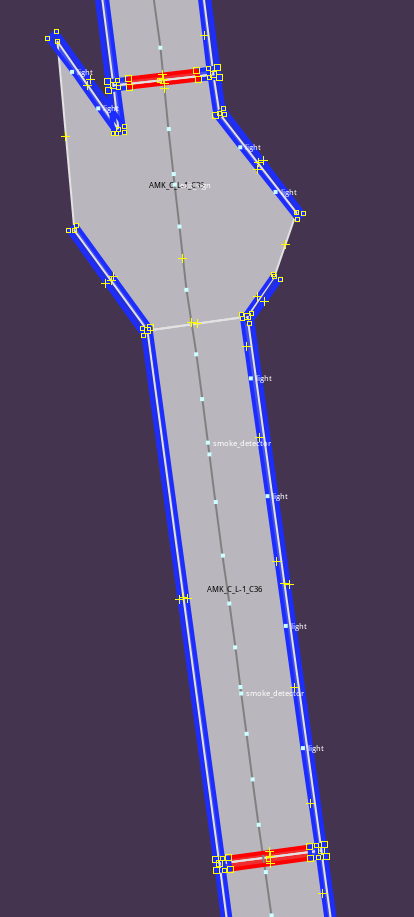
\includegraphics[width=0.5\linewidth]{uitwerking/kaart.png}
    \caption{Grafische voorstelling semantische kaart}
    \label{fig:kaart}
\end{figure}

Het \gls{osm} formaat definieert alles met behulp van nodes. Elke node kan beschikken over een aantal tags waarin sleutel-waarde gegevens gelinkt kunnen worden aan de nodes.
\gls{osm} is een formaat dat gebruikt wordt voor andere doeleinden dan deze toepassing, daarom hebben we gekozen om de nodes op maat gemaakte tags toe te kennen
die onze eigen parser later kan interpreteren.
Aan de kaart zijn een aantal dingen toegevoegd om deze later te kunnen gebruiken.
De objecten zijn als tag toegevoegd via een map editor, en de tags zijn ingevuld in een vast patroon. Het resultaat van deze aanpassing in XML is weergegeven in listing~\ref{lst:object_node}.
De belangrijkste gegevens zijn het type en de name tag, deze geven weer dat het gaat over een 'object' met als label 'licht'.
Alle gegevens in de node tag zelf zijn ge cre\"{e}ert door de map editor bij het aanmaken van de node, waarbij 'lat' en 'lon' de wereldco\"{o}rdinaten zijn van de node.

\lstset{language=XML, caption={XML voorstelling van 1 object node}, label={lst:object_node}}
\begin{lstlisting}[basicstyle=\small]
<node id='137883' action='modify' visible='true' lat='51.068085' lon='4.500029'>
    <tag k='id' v='19' />
    <tag k='name' v='licht' />
    <tag k='type' v='object' />
</node>
\end{lstlisting}

Een 2de aanpassing aan de kaart is de beschrijving van een te volgen route in het midden van de gangen.
Een route bestaat uit een opeenvolging van nodes die aan elkaar grenzen.
Een aantal van deze nodes zijn toegevoegd om discrete locaties te verkrijgen die op 1 route liggen.
De XML structuur van een locatie node is zichtbaar in listing~\ref{lst:location_node}.
Een locatie node is gekenmerkt door een type='location' en bezit een aantal extra tags.

De extra tags zijn het belangrijkste onderdeel van de kaart, zij bevatten informatie over de objecten die zichtbaar zijn van op een specifieke locatie.
Zo geeft bijvoorbeeld een tag met de sleutel $21$ en waarde $10.5$ aan dat object $21$ zichtbaar is onder een hoek van ongeveer $10.5\textdegree$.

\lstset{language=XML, caption={XML voorstelling van 1 lokatie node}, label={lst:location_node}}
\begin{lstlisting}[basicstyle=\small]
<node id='137973' action='modify' visible='true' lat='51.068085' lon='4.500029'>
    <tag k='id' v='27' />
    <tag k='type' v='location' />
    <tag k='20' v='20' />
    <tag k='21' v='10.5' />
</node>
\end{lstlisting}

Een route of 'way' in \gls{osm} is een gesorteerde lijst van alle node id's die op de route liggen. Dit wordt gebruikt om het pad dat de robot zal volgen aan te geven.
In listing~\ref{lst:way} is in XML formaat een deel van de route beschreven.
De aangemaakte locatie nodes zijn via de map editor gekoppeld in \'{e}\'{e}n route, deze route zal ingelezen worden door het programma, en is de enige route die de robot kan afleggen.

\lstset{language=XML, caption={XML voorstelling van een route}, label={lst:way}}
\begin{lstlisting}[basicstyle=\small]
<way id='140546' action='modify' visible='true'>
    <nd ref='4427' />
    <nd ref='137973' />
    <nd ref='137925' />
</way>
\end{lstlisting}

Het inlezen van het \gls{osm} kaartformaat gebeurt via een zelfgemaakte parser die de object, locatie en route nodes inleest in een gelinkte datastructuur
zodat het eenvoudig is om later te verwerken.
De kaart kan gevisualiseerd worden met behulp van een Python \gls{osm} bibliotheek\footnote{https://github.com/gboeing/osmnx}.


\section{Robot positie tracking}\label{sec:lokalisatie}
Nu we alle stappen afzonderlijk besproken hebben, is het tijd om alles te combineren tot \'{e}\'{e}n geheel.
Zoals in figuur~\ref{fig:pipeline1} al weergegeven werd, worden de input beelden van de camera frame per frame verwerkt.
E\'{e}n input afbeelding wordt eerst geanalyseerd door de YOLO object detector waarna het perspectiefpunt gedetecteerd kan worden.
Het perspectiefpunt zou in principe ongeveer het midden van het beeld moeten aangeven.
Dit is echter niet altijd het geval omdat de robot geroteerd kan zijn ten opzichte van de gang.
Daarom wordt er een correctiefactor berekend om het perspectiefpunt ongeveer in het midden van het beeld te leggen.

De 2 detectieresultaten kunnen vervolgens gecombineerd worden om de omgevingsmeting uit te voeren zoals beschreven in hoofdstuk~\ref{sec:omgevingsmeting}.
Dit geeft als resultaat een lijst van gedetecteerde objecten samen met de hoek waaronder ze zichtbaar zijn.

\begin{figure}[t]
    \centering
    \includegraphics[width=\linewidth]{uitwerking/pipeline2.png}
    \caption{Overzicht van de lokalisatie}
    \label{fig:pipeline2}
\end{figure}

De omgevingsmeting en de gegevens beschreven op de semantische kaart moeten nu aan elkaar gelinkt worden om de actuele locatie van de robot te bepalen.
We gaan er vanuit dat de robot vertrekt op een gekende locatie, deze locatie is \'{e}\'{e}n van de discrete locaties aangeduid op de kaart in hoofdstuk~\ref{sec:sem_kaart}.
De eerste vorm van kennis ingebracht in de implementatie is het feit dat de robot niet kan springen, met andere woorden de robot kan enkel op of tussen 2 discrete locatie punten op de kaart zijn.
In het programma wordt dus enkel getracht om de huidige locatie te onderscheiden tussen de vorige locatie node, en de volgende locatie node op de gedefinieerde route.
Figuur~\ref{fig:pipeline2} geeft het overzicht van hoe de lokalisatie verloopt.

Voor elk van deze 2 mogelijke nodes wordt vervolgens een score berekend, deze score geeft aan hoeveel de theoretische node lijkt op de omgevingsmeting van het huidige frame.
Om deze score te berekenen, wordt er eerst geprobeerd om per object-klasse objecten van op de kaart te linken aan objecten uit de omgevingsmeting.
Dit gebeurt door de hoeken te vergelijken.
De objecten waarvan de detectie en de data hoeken het dichtst bij elkaar liggen worden gelinkt.
Uiteraard zijn de metingen niet exact gelijk aan de data, daarom wordt er een afwijking tot 20\% toegestaan bij het linken.

De score die de gelijkenis tussen de meting en data weergeeft wordt berekend op basis van deze gelinkte gegevens.
Elk object uit de node data dat niet gelinkt kon worden met een detectie wordt afgestraft, en elke match wordt beloond.
Vervolgens wordt per match het verschil in hoek (fout) tussen de detectie en data hoek afgetrokken van de score.
De laatste stap is het wegen van de verschillende features. Objecten dichtbij hebben een veel grotere detectiehoek, die nauwkeuriger berekend kan worden.
Daarom wordt er op basis van de hoek een wegingsfactor toegevoegd voor dat specifieke object ten opzichte van de score.
Objecten veraf die misschien nauwelijks zichtbaar zijn die niet gedetecteerd worden straffen zo bijvoorbeeld minder af dan een object dat dichtbij is en zeker gedetecteerd had moeten worden.

Objecten die in het midden van het beeld staan zoals de rookmelders hebben een horizontale hoek van zo goed als 0.
Dit is dus weinig bruikbaar.
Daarom kan er voor dit soort situaties ongeveer dezelfde techniek toegepast worden maar dan in de verticale richting.
De hoek in de verticale richting geeft dan een goede schatting van de afstand tot het object dat zich vlak voor ons bevindt.

De berekening van de score kan worden samengevat in formule~\ref{eq:score} waarbij $a$ de positieve beloningsfactor is, $b$ de negatieve afstraffactor,
$\alpha_{mi}$ is een hoek uitgelezen van de semantische kaart en $\alpha_{di}$ een door detectie gemeten hoek.
$n$ staat voor het aantal links tussen detectie en data hoeken en $m$ is het aantal niet gelinkte objecten.
Met andere woorden $n + m$ is het totaal aantal objecten zichtbaar op de discrete locatie van de kaart.
Functie~\ref{eq:score_weights} genereert de wegingsfactor van de invloed van een object op de score, zoals eerder besproken krijgen objecten met grote hoeken
een grotere invloed op de score.

Deze score wordt berekend voor de 2 kandidaat locaties, en de node met de hoogste score wordt beschouwd als de actuele locatie.
Vervolgens wordt een nieuw input frame verwerkt, en zal de berekening opnieuw beginnen.

\begin{equation}\label{eq:score}
    score = \sum_{i=1}^{n}\big[a - |\alpha_{mi} - \alpha_{di}|\big] \cdot f_w(\alpha_{mi}) + \sum_{i=1}^{m}\big[b \cdot f_w(\alpha_{mi})\big]
\end{equation}

\begin{equation}\label{eq:score_weights}
    f_w(\alpha) = \left\{\begin{array}{lr}
                1 & \text{for } 30 < |\alpha|\\
                \frac{7\alpha + 10}{220} & \text{for } 0 \leq |\alpha| \leq 30\\
    \end{array}
    \right\}
\end{equation}